\section{Conceptual Modelling}\label{sec:cm}
In software development, conceptual data modeling is a concept that represents the relationships between different entities in a database. This data model is generated as a result of the requirement analysis and is the most basic type of data modeling. Therefore, this paradigm, which is known as extremely abstract, is easy to understand by any technician or non-technical person. In this data model, the entity's attributes may or may not be present. Business stakeholders and data architects are frequently involved in the creation of this data model. 
We analyzed our project requirements and developed a very basic data model (Conceptual Data Model), which is shown below.
\begin{figure}[H]
	\captionsetup[subfigure]{labelformat=empty}
	\hfill
		\subfloat{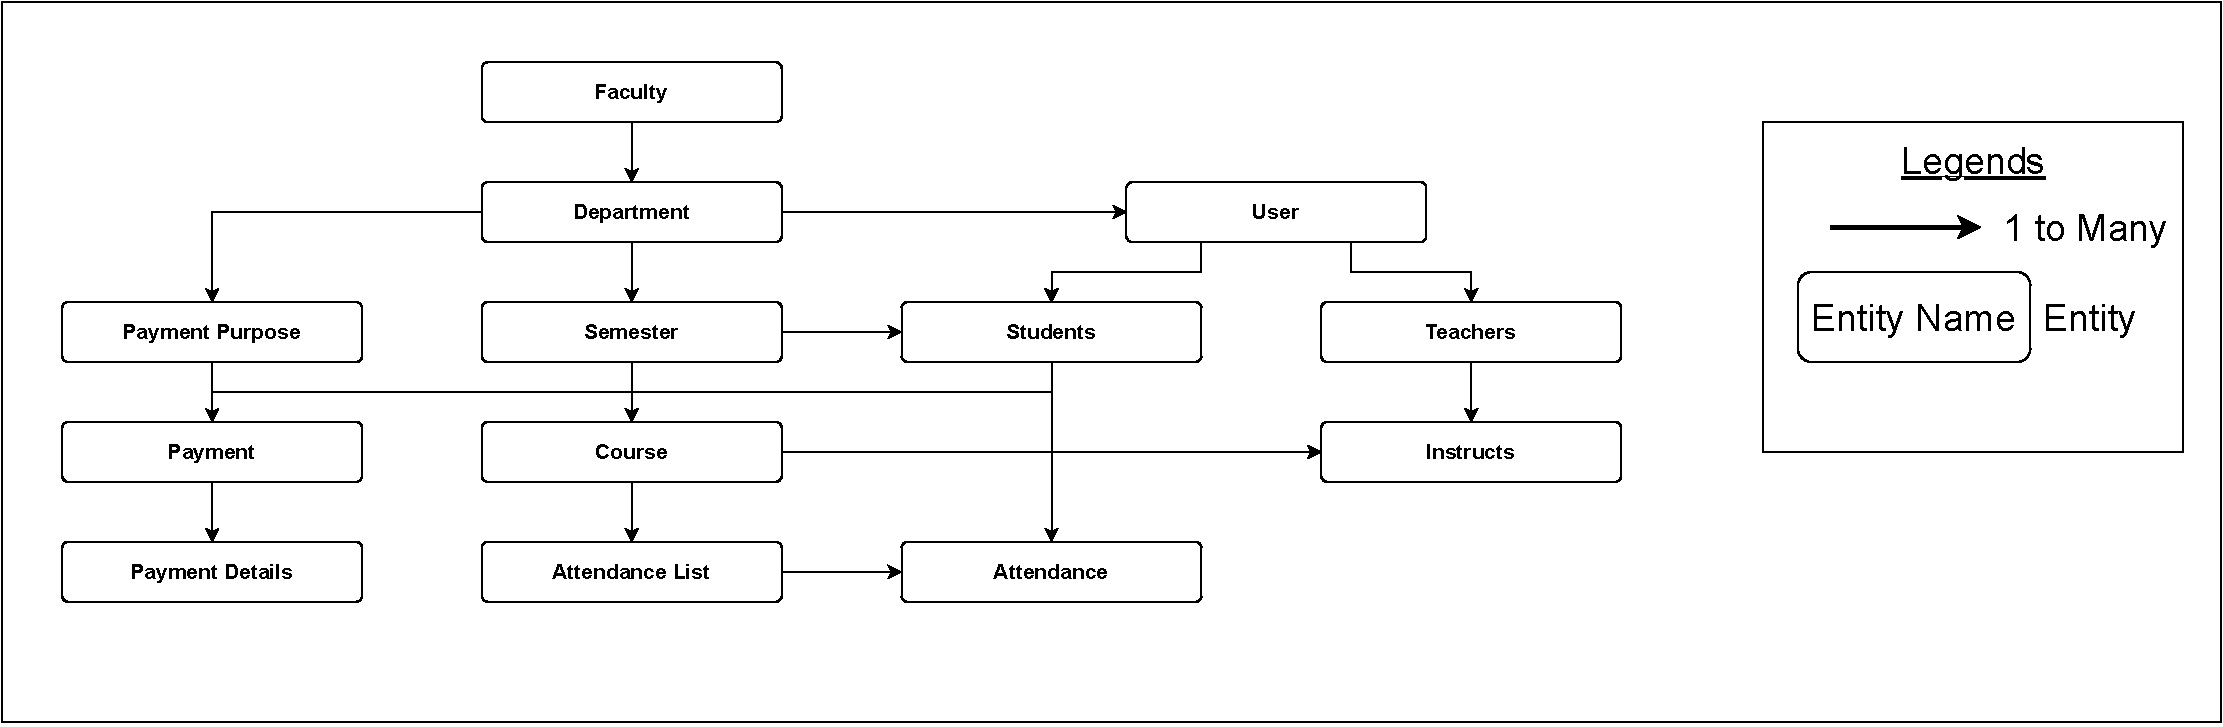
\includegraphics[width=0.7\textwidth]{images/conceptual}}
	\hfill
		\subfloat{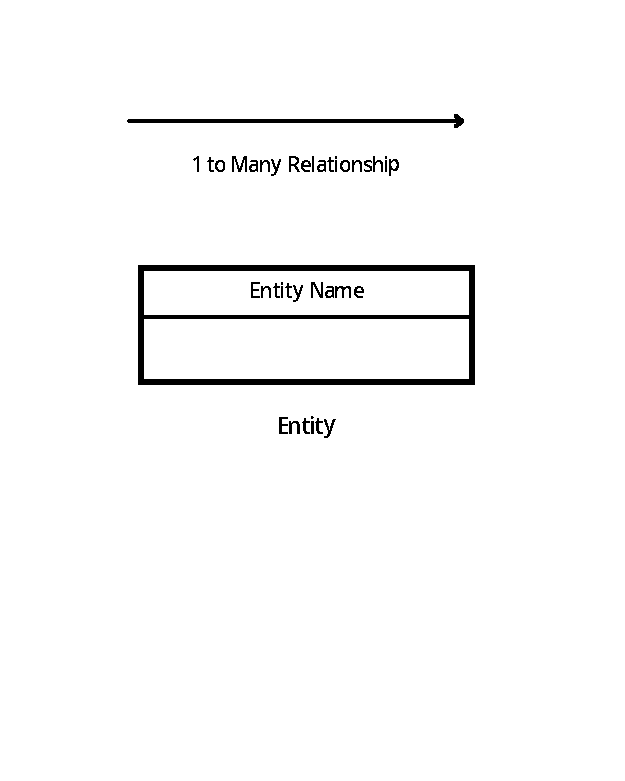
\includegraphics[width=0.3\textwidth]{images/legend}}
	\hfill
	\caption{Conceptual Data Model of CU-OPAS}
\end{figure}
Conceptually model your database using an E-R diagram. Use the legends in your diagram. Write how you find the entity types, relationships, and attributes from Section~\ref{sec:rga}